\begin{frame}{Geometric and topological computing}
\protect\hypertarget{geometric-and-topological-computing}{}

\framesubtitle{rethinking some foundations}

\begin{columns}[T]
\begin{column}{0.48\textwidth}
Complexity of geometric information stems from dramatic increase in
\emph{size}, \emph{diversity}, and \emph{complexity} of
\textbf{geometric data}:

\begin{itemize}
\tightlist
\item
  point clouds,
\item
  boundary meshes,
\item
  NURBs representations,
\item
  finite element meshes,
\item
  CT scans,
\item
  and so on
\end{itemize}
\end{column}

\begin{column}{0.48\textwidth}
Emerging applications (e.g. \textbf{medical 3D}) require the
\textbf{convergence of data structures} from:

\begin{itemize}
\tightlist
\item
  3d computer imaging
\item
  computer graphics
\item
  solid modeling
\item
  computer-aided geometric design
\item
  discrete meshing of domains
\item
  physical simulations
\end{itemize}
\end{column}
\end{columns}

The goals of \emph{unification}, \emph{scalability}, and
\emph{distributed computing} call for \emph{rethinking some foundations}
of geometric and topological computing

\end{frame}

\begin{frame}{Motivation for a new start}
\protect\hypertarget{motivation-for-a-new-start}{}

\begin{columns}[T]
\begin{column}{0.48\textwidth}
\begin{block}{Quad-edge data structure \cite{Guibas1985}}

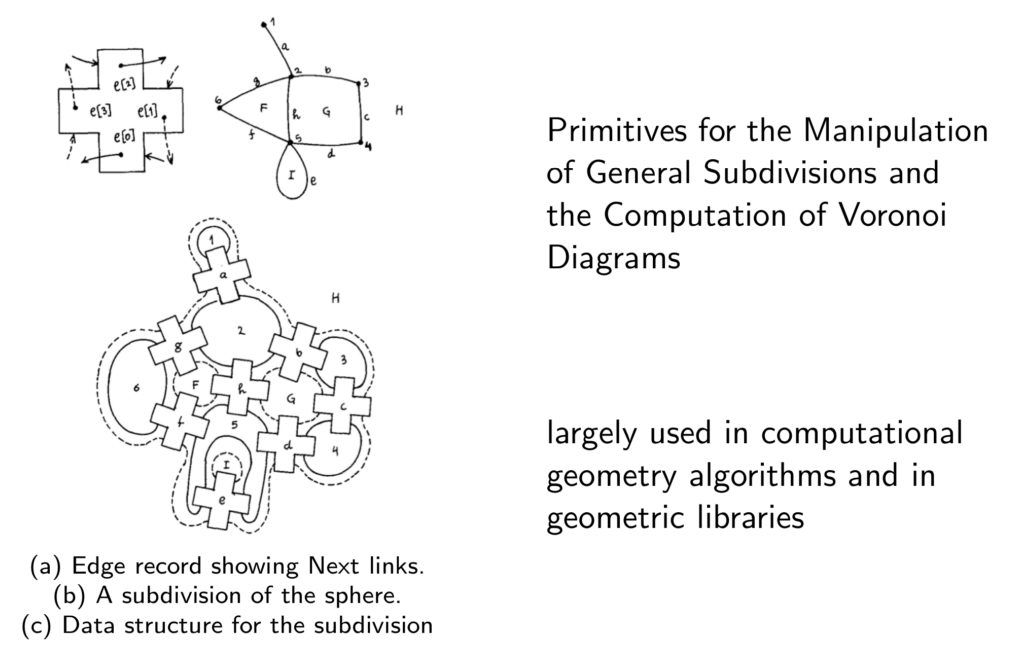
\includegraphics{figs/Guibas1985_quad_edge.png}~

\end{block}

\begin{block}{Hybrid Edge data sturcture \cite{Kalay1989}}

a topological data structure for vertically integrated geometric
modelling

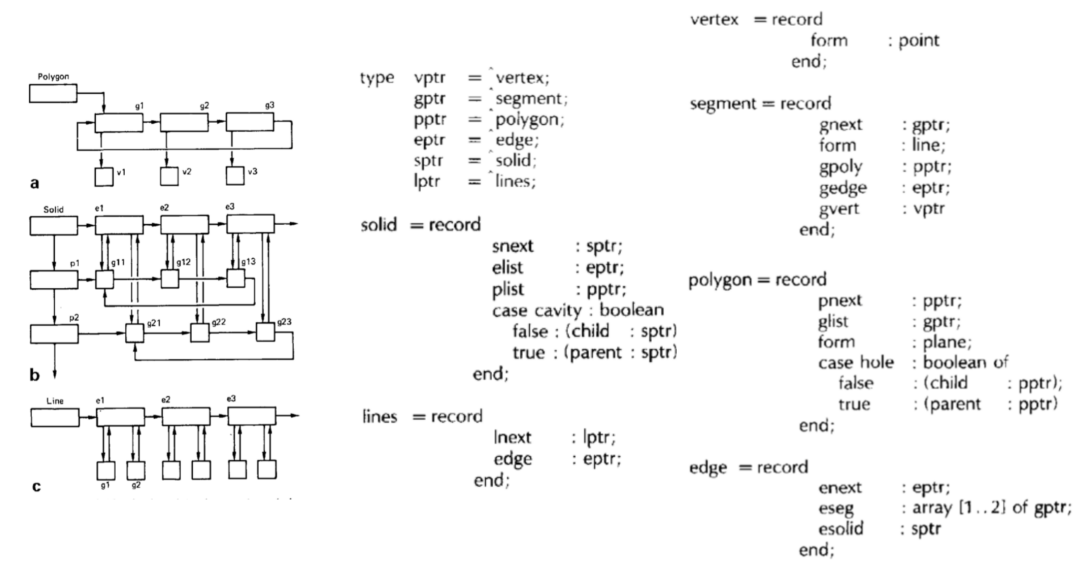
\includegraphics{figs/Kalay1989_hybrid_edge.png}~

\end{block}
\end{column}

\begin{column}{0.48\textwidth}
\begin{block}{Partial-Entity data structure \cite{SangHunLee2001}}

Compact Non-Manifold Boundary Representation Based on Partial
Topological Entities
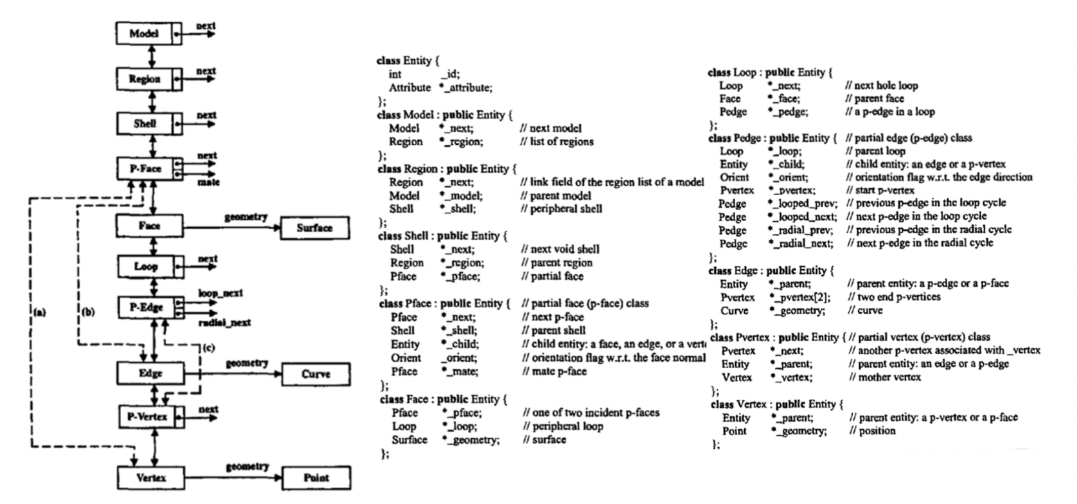
\includegraphics{figs/SangHunLee2001_partial_entity.png}~

\end{block}

\begin{block}{Coupling Entities data structure
\cite{yamaguchi1995nonmanifold}}

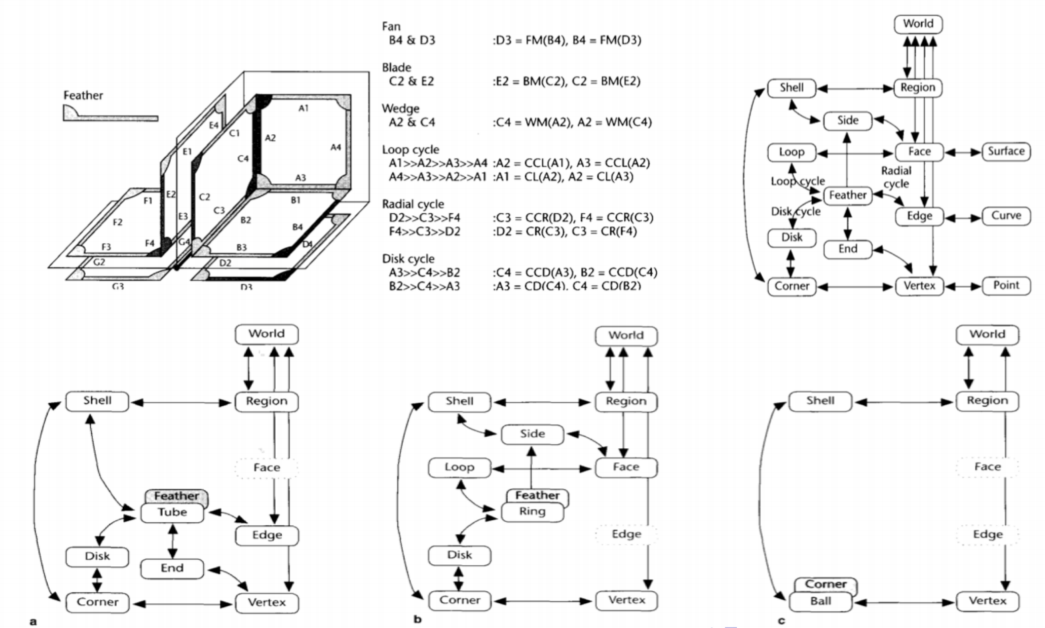
\includegraphics{figs/yamaguchi1995nonmanifold.png}~

\end{block}
\end{column}
\end{columns}

\begin{block}{first sub}

\begin{itemize}
\tightlist
\item
  asdf
\item
  neks
\end{itemize}

\end{block}

\begin{block}{second sub}

\begin{itemize}
\tightlist
\item
  asf
\item
  woens
\end{itemize}

\end{block}

\end{frame}

\begin{frame}{third slide}
\protect\hypertarget{third-slide}{}

asdfa sd asd fas

\end{frame}

\begin{frame}{My slide}
\protect\hypertarget{my-slide}{}

\begin{block}{First column}

contents

\end{block}

\begin{block}{Second column}

contents

\end{block}

\end{frame}
